% Title: glps_renderer figure
% Creator: GL2PS 1.3.8, (C) 1999-2012 C. Geuzaine
% For: Octave
% CreationDate: Mon Nov 16 16:43:05 2015
\setlength{\unitlength}{1pt}
\begin{picture}(0,0)
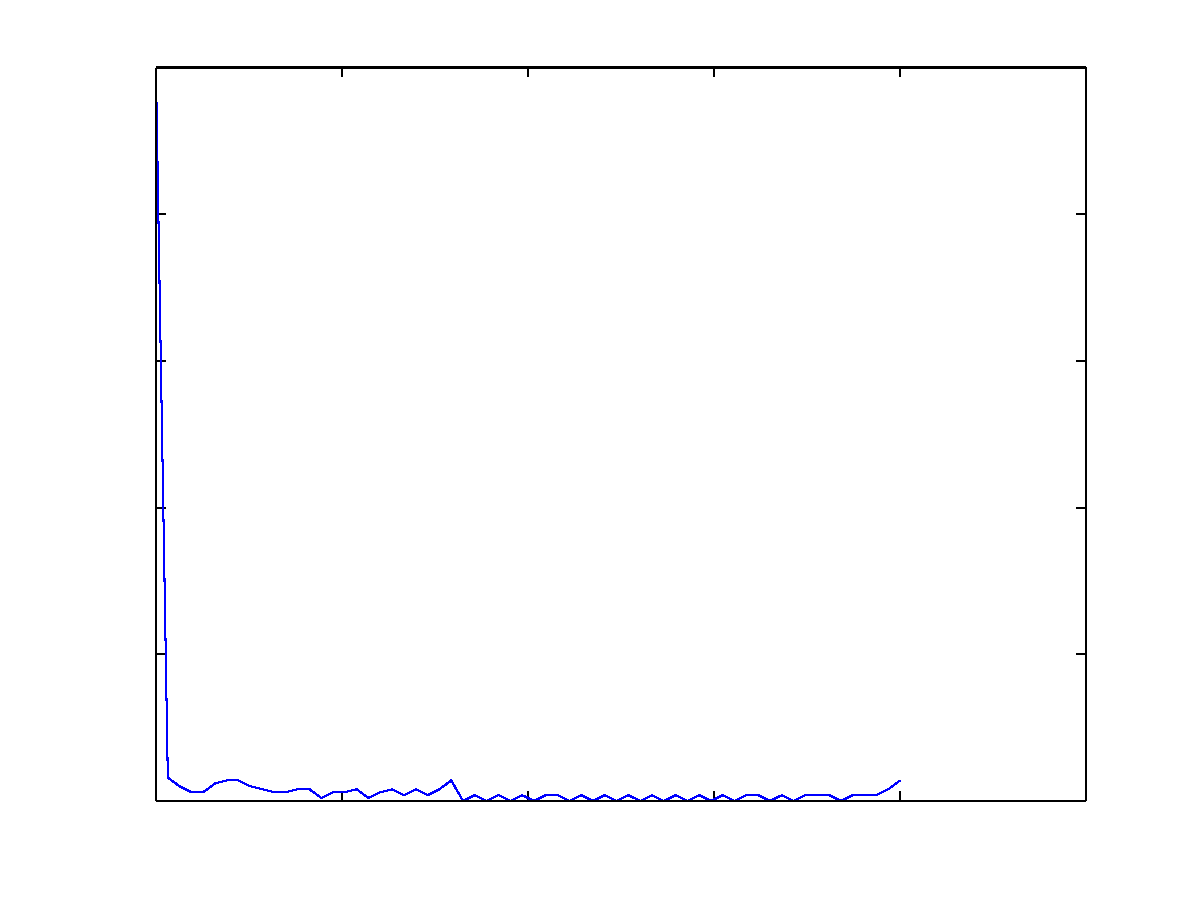
\includegraphics{y_quadriple_hist-inc}
\end{picture}%
\begin{picture}(576,432)(0,0)
\fontsize{12}{0}
\selectfont\put(74.8799,42.519){\makebox(0,0)[t]{\textcolor[rgb]{0,0,0}{{0}}}}
\fontsize{12}{0}
\selectfont\put(164.16,42.519){\makebox(0,0)[t]{\textcolor[rgb]{0,0,0}{{5}}}}
\fontsize{12}{0}
\selectfont\put(253.44,42.519){\makebox(0,0)[t]{\textcolor[rgb]{0,0,0}{{10}}}}
\fontsize{12}{0}
\selectfont\put(342.72,42.519){\makebox(0,0)[t]{\textcolor[rgb]{0,0,0}{{15}}}}
\fontsize{12}{0}
\selectfont\put(432,42.519){\makebox(0,0)[t]{\textcolor[rgb]{0,0,0}{{20}}}}
\fontsize{12}{0}
\selectfont\put(521.28,42.519){\makebox(0,0)[t]{\textcolor[rgb]{0,0,0}{{25}}}}
\fontsize{12}{0}
\selectfont\put(69.8755,47.52){\makebox(0,0)[r]{\textcolor[rgb]{0,0,0}{{0}}}}
\fontsize{12}{0}
\selectfont\put(69.8755,117.936){\makebox(0,0)[r]{\textcolor[rgb]{0,0,0}{{50}}}}
\fontsize{12}{0}
\selectfont\put(69.8755,188.352){\makebox(0,0)[r]{\textcolor[rgb]{0,0,0}{{100}}}}
\fontsize{12}{0}
\selectfont\put(69.8755,258.768){\makebox(0,0)[r]{\textcolor[rgb]{0,0,0}{{150}}}}
\fontsize{12}{0}
\selectfont\put(69.8755,329.184){\makebox(0,0)[r]{\textcolor[rgb]{0,0,0}{{200}}}}
\fontsize{12}{0}
\selectfont\put(69.8755,399.6){\makebox(0,0)[r]{\textcolor[rgb]{0,0,0}{{250}}}}
\fontsize{12}{0}
\selectfont\put(298.08,31.519){\makebox(0,0)[t]{\textcolor[rgb]{0,0,0}{{Intensity}}}}
\fontsize{12}{0}
\selectfont\put(47.8755,223.56){\rotatebox{90}{\makebox(0,0)[b]{\textcolor[rgb]{0,0,0}{{Count}}}}}
\fontsize{12}{0}
\selectfont\put(298.08,409.6){\makebox(0,0)[b]{\textcolor[rgb]{0,0,0}{{Histogram of $Y_{quadriple}$}}}}
\end{picture}
